\chapter{Progetto}
\label{cha:experience}

\section{Ontopic}
\label{sec:ontopic}
Il tirocinio da me svolto è avvenuto presso l'azienda Ontopic s.r.l. Tale azienda è nata nel 2019 come spin-off della Libera Università di Bolzano dal prof. Diego Calvanese insieme al professore Marco Montali, i ricercatori Guohui Xiao e Benjamin Cogrel
e l’amministratore delegato Peter Hopfgartner presso il NOI Techpark di Bolzano\cite{Ontopic}.

L'azienda nasce con lo scopo di proporre soluzioni di data integration basate, in particolare, sull'integrazione semantica come i Virtual Knowledge Graph. Ontopic fornisce sia consulenza diretta ad aziende con soluzioni ad-hoc
per integrazione ed analisi dati che una soluzione proprietaria per il mapping di VKG chiamata Ontopic Studio. Questo applicativo è basato sul Virtual Knowledge Graph system Ontop, del quale Ontopic è uno dei principali contributori, 
e permette di realizzare mapping in modo efficiente tramite un interfaccia grafica no-code semplice e che ne permette quindi l'uso anche a persone senza un background in tecniche semantiche. \cite{OntopicStudio}

\section{Il modulo bi-connector}
\label{sec:bi-connector}
Durante la mia esperienza di tirocinio presso Ontopic, ho lavorato all'interno del progetto bi-connector. Tale modulo ha lo scopo di permettere all'utente finale di interrogare un VKG non solo tramite query SPARQL, come di consuetudine, ma anche
tramite strumenti di Business Intelligence (BI) come Tableau, PowerBi o Qlik.
Mentre questi applicativi presentano nativamente connettori verso molteplici fonti di dati tra cui: la maggior parte dei database relazionali, database NoSQL come MongoDB, fogli Excel,
dati in formato JSON, file PDF, connessioni personalizzate tramite JDBC o ODBC, \dots, non forniscono invece connettori nativi per i VKG ed è proprio per questo che nasce bi-connector.

Nel resto dell'elaborato farò riferimento principalmente a Tableau, piuttosto che PowerBI e Qlik, in quanto è lo strumento di BI sul quale si è concentrato lo sviluppo durante il mio periodo di permanenza presso Ontopic.

Possiamo pensare a bi-connector come costituito di due parti principali: una che si occupa della costruzione di un database, a partire da un'ontologia, che possa essere connesso allo strumento di BI target e una seconda parte che ha il compito di tradurre le query
SQL sul database in una forma equivalente e comprensibile dal VKG sottostante.

\subsection{Creazione database}
\label{sec:bi-connector_db}
A partire dal nostro VKG è possibile definire un insieme di viste SPARQL. 
dove ognuna di queste viste corrisponde ad un'associazione tra una query SELECT SPARQL e un nome che ne descrive il risultato restituito. Ad esempio la vista seguente:
\begin{verbatim}
[[schemas.views]]
    name="prof"
    query="""
        PREFIX : <http://university.example.org/>
        SELECT * WHERE {
        ?id a :Professor ; :firstName ?fName ; :lastName ?lName .
        }
    """
\end{verbatim}
assegna il nome \textit{prof} all'insieme di dati il cui \textit{id} è di classe Professor e che ha come attributi \textit{firstName} e \textit{lastName}.

Queste viste vengono convertite in delle viste relazioni le quali costituiscono il database PostgreSQL che usiamo per connetterci a strumenti di BI.

La parte più complessa della traduzione risulta essere la gestione dei tipi. Infatti, SPARQL è basato su tipizzazione dinamica il che significa che tipi diversi possono essere usati per la stessa colonna, mentre SQL usa 
tipizzazione statica. Tutte le viste per le quali non è possibile determinare il tipo finale prima della traduzione vengono quindi scartate.

\subsection{Parsing di query SQL}
\label{sec:bi-connector_parsing}
\`E possibile interrogare il database inizialmente creato tramite query SQL, ma queste devono poi essere tradotte in una rappresentazione comprensibile dal VKG sottostante. Infatti, le query non sono eseguite sul database da noi creato, ma sul
VKG originale così da poterne sfruttare le capacità di inferenza.

In quanto il VKG system utilizzato è Ontop, le query SQL vengono tradotte in un albero IQ, descritto precedentemente anche nella sezione \ref{sec:ontop_iq}.

Inizialmente, le query delle quali era possibile fare il parsing erano quasi esclusivamente del tipo SELECT-JOIN-WHERE, ovvero un'unione di query congiuntive. Questo era dovuto al fatto che il parser SQL in uso fosse quello nativo di Ontop,
il quale ha come scopo principale la traduzione dei mapping che sono, nella maggior parte dei casi, rappresentabili tramite questo tipo di semplici query.
A causa di questa limitazione moltissime delle query generate automaticamente da strumenti di Business Intelligence dovevano essere riscritte in una forma semplifica per poter essere eseguite.
Di seguito un esempio in cui la query è semplificata eliminando il LEFT JOIN e l'ORDER BY in quanto non supportati.
\begin{verbatim}
    SELECT n.oid, n.*, d.description 
    FROM pg_catalog.pg_namespace n
    LEFT OUTER JOIN pg_catalog.pg_description d ON d.objoid=n.oid 
        AND d.objsubid=0 AND d.classoid='pg_namespace'::regclass
    ORDER BY nspname
\end{verbatim}    
diventa:
\begin{verbatim}
    SELECT n.* 
    FROM pg_catalog.pg_namespace n;
\end{verbatim}

Date queste limitazioni, si è deciso di adottare un parser diverso ovvero JSqlParser. JSqlParser è un parser di istruzioni SQL
che trasforma una query in una gerarchia di classi Java. \`E basato sul visitor pattern il quale permette di separare in modo semplice un algoritmo dalla struttura dati sulla quale è utilizzato.
In altre parole, questo pattern rappresenta un'operazione che deve essere eseguita su un insieme eterogeneo di oggetti e, per ognuno di questi, potrebbe dover essere implementata in modo differente \cite{JSqlParser}.

\section{Prime attività}
\label{sec:prerequisits}
La prima attività svolta all'interno del tirocinio è stata quella di familiarizzare con le tecnologie legate ai VKG che mi sarebbero servite in seguito. In particolare ho svolto
il tutorial introduttivo ad Ontop tramite la piattaforma Protege così da provare direttamente cosa significhi tradurre fonti di dati in un'ontologia tramite mapping.

Il mio compito principale è stato quello di estendere il parser SQL in uso così da supportare un numero maggiore di costrutti. Come affermato anche precedentemente, il parser inizialmente utilizzato era
esclusivamente in grado di tradurre semplici query il che è risultato essere insufficiente affinché potesse essere usato da strumenti di Business Intelligence in modo non banale.

\`E stato quindi analizzato quali fossero i costrutti maggiormente presenti nelle query generate automaticamente dagli strumenti di BI, di cui un esempio sopra nella sezione \ref{sec:bi-connector_parsing}. Tra questi
i principali sono sicuramente il GROUP BY per l'aggregazione, dato anche lo scopo degli strumenti di BI di fornire informazioni d'insieme sull'intero dataset, e l'ORDER BY che
permette di modificare l'ordinamento dei dati in base a parametri arbitrari.

\subsection{Database di riferimento}
Durante la durata del tirocinio, tutte le funzionalità implementate sono state testate su un semplice VKG con un database relazionale H2 come sorgente che rappresenta alcune informazioni riguardanti professori universitari.
I test sono stati eseguiti sia all'interno della codebase stessa grazie al framework JUnit che tramite il client SQL DBeaver che ha permesso la visualizzazione del database PostgreSQL creato dal bi-connector e la sua
interrogazione diretta.
Di seguito si descrivono le tabelle (\ref{tab:prof} \ref{tab:profstats}, \ref{tab:course}, \ref{tab:teaching}) di questo database che sono inoltre quelle a cui si farà riferimento in tutti i frammenti di codice successivi.
\begin{table}[ht]
    \caption{Tabella prof}
    \label{tab:prof}
    \centering
    \begin{tabular}{ | c | c | c | }
        \hline
        id                                         & fName   & lName   \\ \hline
        http://university.example.org/professor/10 & Roger   & Smith   \\ \hline
        http://university.example.org/professor/20 & Frank   & Pitt    \\ \hline
        http://university.example.org/professor/30 & John    & Deep    \\ \hline
        http://university.example.org/professor/40 & Micheal & Jackson \\ \hline
        http://university.example.org/professor/50 & Diego   & Gamper  \\ \hline
        http://university.example.org/professor/60 & Johann  & Helmer  \\ \hline
        http://university.example.org/professor/70 & Barbare & Dodero  \\ \hline
        http://university.example.org/professor/80 & Mary    & Poppins \\ \hline
    \end{tabular}
\end{table}

\begin{table}[ht]
    \caption{Tabella prof\_stats}
    \label{tab:profstats}
    \centering
    \begin{tabular}{| c | c | c |}
        \hline
        profId                                     & totalStudents & countCourse \\ \hline
        http://university.example.org/professor/10 & 21            & 2           \\ \hline
        http://university.example.org/professor/30 & 12            & 1           \\ \hline
        http://university.example.org/professor/80 & 13            & 1           \\ \hline
    \end{tabular}
\end{table}

\begin{table}[ht]
    \caption{Tabella course}
    \label{tab:course}
    \centering
    \begin{tabular}{| c | c | c |}
        \hline
        id                                                       & duration & nbStudents \\ \hline
        http://university.example.org/course/LinearAlgebra       & 24.5     & 10         \\ \hline
        http://university.example.org/course/DiscreteMathematics & 30       & 11         \\ \hline
        http://university.example.org/course/AdvancedDatabases   & 20       & 12         \\ \hline
        http://university.example.org/course/ScientificWriting   & 18       & 13         \\ \hline
    \end{tabular}
\end{table}

\begin{table}[H]
    \small
    \caption{Tabella teaching}
    \label{tab:teaching}
    \centering
    \begin{tabular}{| c | c | }
        \hline
        teacher                                    & course                                                   \\ \hline
        http://university.example.org/professor/30 & http://university.example.org/course/AdvancedDatabases   \\ \hline
        http://university.example.org/professor/10 & http://university.example.org/course/DiscreteMathematics \\ \hline
        http://university.example.org/professor/10 & http://university.example.org/course/LinearAlgebra       \\ \hline
        http://university.example.org/professor/80 & http://university.example.org/course/ScientificWriting   \\ \hline
    \end{tabular}
\end{table}

Inoltre, dato il fatto che ogni DBMS tende ad avere un proprio dialetto SQL, è stato molto importante assicurarsi che i costrutti da me implementati ricalcassero il
comportamento presente in PostgreSQL e, nel caso ciò non fosse possibile, fornire messaggi d'errore di facile comprensione. Ad esempio, la funzione CONCAT() 
è null-rejecting in PostgreSQL, ovvero tutti gli argomenti pari a NULL sono ignorati, mentre in altri dialetti, come ad esempio MySQL, se uno degli argomenti è NULL allora il risultato
della concatenazione è anch'esso NULL.
Al fine di aiutarmi in ciò, ho utilizzato la documentazione di PostgreSQL e, per test più pratici, DBFiddle, uno strumento online per testare in modo veloce, e
senza bisogno di alcun setup, frammenti di codice SQL.


\section{Costrutti implementati}
\label{sec:implementation}
La struttura usata per il parsing è basata sulla classe \textit{IQTreeExpression.java} la quale è composta da:
\begin{itemize}
    \item IQTree: albero composto di nodi IQ. Tale albero viene costruito partendo dalle foglie e viene esteso aggiungendo nuovi nodi come radici dell'albero stesso. Da un punto di vista
          più pratico abbiamo come foglie degli extensional node che rappresentano le tabelle elencate all'interno della query e al di sopra di esse sono presenti altri nodi che
          rappresentano le varie operazioni eseguite.
    \item RAExpressionAttributes: dizionario che contiene le colonne delle tabelle coinvolte nella query e tutti gli alias ad esse associati. Per alias si intendono sia nomi definiti
          dall'utente tramite la keyword AS o come nome di una tabella, sia quelli definiti internamente al codice al fine di assicurarne l'univocità.
\end{itemize}
Di seguito un esempio di un IQTreeExpression generato dalla query
\begin{verbatim}
    SELECT "id", "fName", "lName"
    FROM prof p

    IQTreeExpression{
        iqTree = EXTENSIONAL "prof_views"."prof"(0:id1,1:fName1,2:lName1), 
        raExpressionAttributes=attributes: {"id"=id1, p."id"=id1, 
         "fName"=fName1, p."fName"=fName1, "lName"=lName1, p."lName"=lName1} 
         with {"id"=[p], "fName"=[p], "lName"=[p]}
    } 
    \end{verbatim}

\subsection{Modificatori di cardinalità}
I primi costrutti da essere implementati sono stati quelli responsabili della modifica della cardinalità di una tabella ovvero DISTINCT e LIMIT-OFFSET. La loro implementazione
risulta essere abbastanza semplice, ma ciò mi ha permesso di acquisire familiarità con la codebase preesistente e con librerie esterne come JSqlParser
in modo più rapido ,dato che l'implementazione dei costrutti non necessitava di logiche complesse.

\subsubsection*{DISTINCT}
Il costrutto DISTINCT permette di eliminare righe duplicate ed è stato implementato aggiungendo un nodo IQ di tipo distinct.

La clausola DISTINCT ON non è stata invece implementata in quanto non parte dello standard SQL, ma fornita da PostgreSQL. Inoltre non è stata considerata fondamentale in quanto
può essere rimpiazzata tramite l'uso di una subquery o, in alcuni casi, anche tramite aggregazione \cite{PGDistinct}.
\subsubsection*{LIMIT e OFFSET}
Le clausole LIMIT e OFFSET permettono di restringere il numero di righe restituite da una query e di saltare le prime $n$ righe quando queste vengono restituire rispettivamente.
Date le loro funzionalità complementari sono spesso usate insieme anche se possono essere usate separatamente.
Ad esempio la forma \verb+LIMIT 5 OFFSET 2+ ritorna le prime 5 righe dopo che se ne sono saltate 2.

Anche se supportata dalla maggior parte dei DBMS, e quindi ampiamente usata, la clausola LIMIT non fa parte dello standard SQL. Una possibile alternativa standardizzata è l'utilizzo
della keyword FETCH la cui sintassi è \verb+FETCH { FIRST | NEXT } [ fetch_rows ] { ROW | ROWS }+ \verb+ONLY+ dove FIRST/NEXT e ROW/ROWS sono sinonimi e possono quindi essere usati
in modo intercambiabile \cite{Fetch}.

Al fine di implementarne la funzionalità, sia per LIMIT che per FETCH, è stato usato uno slice node il quale permette di specificare esclusivamente un offset o sia
un limite che un offset.

Inoltre, quando si utilizza LIMIT è consigliato aggiungere anche un ORDER BY che forza un ordine alle righe prima che queste vengano selezionate. Questo assicura che il risultato sia 
lo stesso per esecuzioni successive della stessa query \cite{PGLimit}.

\subsection{Ordinamento righe}
La keyword ORDER BY permette di riordinare le righe risultanti da una query in base a specifiche condizioni, sia in modo ascendente che discendente. Un altro aspetto importante è quello del
NULL ordering, ovvero come i valori NULL sono trattati al fine dell'ordinamento. In PostgreSQL i valori pari a NULL vengono considerati come maggiori di qualsiasi altro valore mentre questo
è l'opposto per gli IQ tree i quali seguono una semantica simile a quella di SPARQL. Quindi gli ordinamenti del tipo \verb+ORDER BY ASC NULLS LAST+ e \verb+ORDER BY DESC NULLS FIRST+
non sono supportati \cite{PGOrderBY}.

L'implementazione dell'ORDER BY è risultata essere relativamente complessa in quanto presenta un'ampia casistica. Ad esempio, si può avere uno o più criteri di ordinamento e
ognuno di essi può essere una colonna o una funzione. Inizialmente il costrutto è stato implementato usando un order by node il quale richiede come argomento una lista di comparatori
dove ogni comparatore è costituito dal termine rispetto al quale si sta effettuando l'ordinamento e se quest'ultimo è ascendente o meno.

Una volta svolti i primi test, è subito emerso un problema riguardante la rinomina delle variabili in quanto una volta che ad una variabile veniva assegnato un alias si andava a perdere
il nome della originale della variabile. Quindi ad esempio un query del tipo:
\begin{verbatim}
    SELECT "fName" as v
    FROM prof p 
    ORDER BY "fName"
\end{verbatim}
avrebbe restituito un errore in quanto l'unica variabile presente a seguito della proiezione sarebbe stata \textit{v} e sarebbe quindi stato impossibile eseguire un ordinamento basato su
\textit{fName}.

Si è quindi deciso di estendere l'implementazione per supportare questo comportamento aggiungendo un construction node che proietta tutte le variabili presenti e tiene traccia delle sostituzioni che
avvengono. Inoltre, al fine di evitare collisioni tra gli attributi non proiettati, che vengono appunto mantenuti in questa versione, e gli alias, tutti gli attributi sono rinominati aggiungendo un
suffisso casuale al nome della variabile stessa. La query vista sopra produce quindi questa IQTreeExpression:
\begin{verbatim}
    IQTreeExpression{
        iqTree=CONSTRUCT [v] []
         ORDER BY [ASC(fName)]
          CONSTRUCT [v, fName, fName1f1611f1-6d9d-4347-9c60-f51bbdc89a09, 
           lName, lName0c931a3d-93fb-406c-b33c-6f4743af211c, id, 
           idf859a5d9-d246-42a2-a62f-e722a1175dc4] [fName/v, 
           idf859a5d9-d246-42a2-a62f-e722a1175dc4/id, 
           lName0c931a3d-93fb-406c-b33c-6f4743af211c/lName, 
           fName1f1611f1-6d9d-4347-9c60-f51bbdc89a09/v]
            CONSTRUCT [id, v, lName] []
             EXTENSIONAL "prof_views"."prof"(0:id,1:v,2:lName), 
        raExpressionAttributes=attributes: {v=v} with {v=[]}
    } 
\end{verbatim}

\`E inoltre possibile una forma del tipo \verb+ORDER BY numerical_constant+ dove la costante numerica presente viene utilizzata come indice della corrispondente colonna proiettata. Tale
uso è scoraggiato in quanto il risultato potrebbe non essere deterministico se si va a cambiare la struttura del database stesso, ma è stato implementato ugualmente in quanto viene
ampiamente usato nelle query generate in modo automatico da Tableau.

\subsection{Combinazione tabelle}
Un'altra parte importante al fine formulare query con risultati non banali, è la possibilità di combinare le informazioni presenti in molteplici tabelle. Personalmente, mi sono occupata
esclusivamente dell'implementazione del LEFT JOIN in quanto CROSS e INNER JOIN erano già entrambi funzionanti nel momento in cui ho iniziato il mio tirocinio.

In particolare, l'operazione di LEFT JOIN estende tutte le righe della prima tabella con i valori di una seconda tabella basandosi su una determinata condizione booleana di join. Tale condizione
può essere espressa in due modi:
\begin{itemize}
    \item \verb+LEFT JOIN ON condition+: in questo caso viene specificata una serie di condizioni, tipicamente di uguaglianza tra due colonne appartenenti a tabelle diverse
    \item \verb+LEFT JOIN USING column+: usato se la colonna rispetto alla quale vogliamo eseguire il join ha lo stesso nome in entrambe le tabelle
\end{itemize}

A fini implementativi, entrambe le condizioni vengono espresse come una ImmutableExpression, ovvero un espressione booleana, la quale viene usata come filtro all'interno di un left join node.
Di seguito un esempio dell'IQTreeExpression e del risultato generato dalla query:
\begin{verbatim}
    SELECT p.id, "fName", "totalStudents"
    FROM prof p
    LEFT JOIN prof_stats ps ON p.id = ps."profId"
\end{verbatim}
la quale produce come IQTreeExpression
\begin{verbatim}
    IQTreeExpression{iqTree=CONSTRUCT [id, fName, totalStudents] []
     CONSTRUCT [id, fName, totalStudents,lName, countCourse, profId,
        variabili generate casualmente per univocità] [elenco 
        sostituzioni come visto precedentemente]
      CONSTRUCT [id, fName, lName, profId, totalStudents, countCourse] []
       LJ STRICT_EQ2(id,profId)
        EXTENSIONAL "prof_views"."prof"(0:id,1:fName,2:lName)
        EXTENSIONAL "prof_views"."prof_stats"(0:profId,1:totalStudents,
            2:countCourse), 
    raExpressionAttributes=attributes: {id=id, "fName"=fName, 
        "totalStudents"=totalStudents} with {id=[], "fName"=[], 
        "totalStudents"=[]}}
\end{verbatim}
ed ha come risultato la tabella \ref{tab:leftJoinOn}.
\begin{table}[ht]
    \centering
    \caption{Tabella LEFT JOIN}
    \label{tab:leftJoinOn}
    \begin{tabular}{ | c | c | c | c | c | c |}
        \hline
        id                                         & fName   & totalStudents \\ \hline
        http://university.example.org/professor/10 & Roger   & 21            \\ \hline
        http://university.example.org/professor/20 & Frank   & NULL          \\ \hline
        http://university.example.org/professor/30 & John    & 12            \\ \hline
        http://university.example.org/professor/40 & Micheal & NULL          \\ \hline
        http://university.example.org/professor/50 & Diego   & NULL          \\ \hline
        http://university.example.org/professor/60 & Johann  & NULL          \\ \hline
        http://university.example.org/professor/70 & Barbare & NULL          \\ \hline
        http://university.example.org/professor/80 & Mary    & 13            \\
        \hline
    \end{tabular}
\end{table}

Questa implementazione non risulta però essere completa in quanto presenta comportamenti non corretti in alcuni casi nei quali le colonne sulle quali viene eseguito il join hanno lo stesso nome.
Ad esempio, la query
\begin{verbatim}
    SELECT p.*, ps.*
    FROM (SELECT id as "profId", "fName", "lName" FROM prof_views.prof p1) p
    LEFT JOIN prof_views.prof_stats ps ON p."profId" = ps."profId"
\end{verbatim}
ritorna un errore in quanto i nomi di due colonne (p.profId e ps.profId) all'interno del SELECT sono uguali. Questa è una limitazione di Ontop stesso il quale non permette di avere variabili
con lo stesso nome all'interno di una proiezione.

Una volta realizzato il LEFT JOIN, l'implementazione del RIGHT JOIN è risultata essere banale in quanto è stato sufficiente invertire i ruoli delle due tabelle sulle quali viene effettuato
il join per ottenere il comportamento corretto.

\subsection{Operazioni insiemistiche}
Gli operatori insiemistici uniscono i risultati di due query in un unico insieme finale. I due insiemi che devono essere uniti devono rispettare alcune condizioni:
devono restituire lo stesso numero di colonne e colonne corrispondenti devono avere tipi compatibili \cite{PGSetOp}. Inoltre, una limitazione aggiuntiva introdotta dalla nostra
implementazione, prevede che colonne corrispondenti debbano avere lo stesso nome.

\subsubsection*{UNION}
L'operazione di UNION aggiunge alle righe risultanti dalla prima query quelle ottenute da una seconda query eliminando i duplicati. Se si vuole mantenere le righe ripetute, è possibile
usare il costrutto UNION ALL.

La sua implementazione prevede l'utilizzo di uno union node, il quale mantiene i duplicati, seguito eventualmente da un distinct node nel caso sia necessario eliminare le copie.

\subsubsection*{EXCEPT}
L'operazione di sottrazione, chiamata in PostgreSQL EXCEPT invece dello standard MINUS, restituisce tutte le righe risultanti dalla prima query che non sono presenti anche nei
risultati della seconda.

La sua implementazione risulta essere particolarmente interessante in quanto non esiste un IQ node che ne imiti di comportamento direttamente. Viene quindi eseguito un left join tra le due
tabelle e tramite un filtro vengono eliminate tutte le righe per le quali le colonne provenienti dalla tabella di destra, identificate grazie colonna ausiliaria \textit{rightProv},
non sono pari a NULL. Infine viene usato un construct node così da mantenere solo le variabili desiderate. Ad esempio la query
\begin{verbatim}
    SELECT "id"
    FROM prof p
    EXCEPT
    SELECT "profId" AS "id"
    FROM prof_stats ps 
\end{verbatim}
ha come risultato la tabella \ref{tab:minus}
\begin{table}[ht]
    \centering
    \caption{Tabella MINUS}
    \label{tab:minus}
    \begin{tabular}{ | c | c | c | c | c | c |}
        \hline
        id                                         \\ \hline
        http://university.example.org/professor/20 \\ \hline
        http://university.example.org/professor/40 \\ \hline
        http://university.example.org/professor/50 \\ \hline
        http://university.example.org/professor/60 \\ \hline
        http://university.example.org/professor/70 \\
        \hline
    \end{tabular}
\end{table}
e produce come l'IQTreeExpression seguente:
\begin{verbatim}
    IQTreeExpression{iqTree=CONSTRUCT [id] []
     FILTER IS_NULL(rightProv)
       LJ
        CONSTRUCT [id] []
         CONSTRUCT [id, fName, lName, variabili generate casualmente per
          univocità] [elenco sostituzioni]
           CONSTRUCT [id, fName, lName] []
            EXTENSIONAL "prof_views"."prof"(0:id,1:fName,2:lName)
        CONSTRUCT [id, rightProv] [rightProv/"TRUE"^^BOOLEAN]
         CONSTRUCT [id] []
          CONSTRUCT [id, totalStudents,countCourse, variabili generate 
           casualmente per univocità] [elenco sostituzioni]
            CONSTRUCT [id, totalStudents, countCourse] []
             EXTENSIONAL "prof_views"."prof_stats"(0:id,1:totalStudents,
             2:countCourse),
    raExpressionAttributes=attributes: {"id"=id} with {"id"=[]}}
\end{verbatim}

Inoltre non è stato possibile implementare l'operazione di EXCEPT ALL in quanto non supportata dalla versione in uso di JSqlParser.

\subsection{Aggregazione}
L'aggregazione è una funzionalità estremamente importante in quanto permette di raggruppare i dati in base a parametri arbitrari ed
ottenere così informazioni riassuntive sui dati.
\subsubsection*{Funzioni di aggregazione}
Le funzioni di aggregazione (SUM, COUNT, MIN, MAX, AVG ) sono molto utili in quanto permettono di esprimere caratteristiche di una colonna, 
o di un'intera tabella, tramite un singolo numero riassuntivo.

Il principale ostacolo alla loro implementazione è stato determinare il tipo della colonna sulla quale la funzione era applicata.
Per questo, inizialmente, si è assunto a priori che tutte le funzioni di aggregazione fossero eseguite su colonne di tipo intero. In un
secondo momento si è implementato invece un meccanismo grazie alla classe \textit{NotYetTypedAggregationFunctionSymbol.java} la quale 
permette di posporre la decisione sul tipo di dato fino a quando questo non è conosciuto dal sistema.

Ad esempio, le due query seguenti applicano la funzione SUM alle colonne \textit{nbStudents} e \textit{duration} le quali sono rispettivamente 
un numero intero e uno decimale ed è possibile vedere ciò nel tipo che viene dato alla funzione all'interno dell'aggregation node.
\begin{verbatim}
    SELECT sum("nbStudents") AS sum
    FROM course c 
\end{verbatim}
produce l'IQTreeExpression:
\begin{verbatim}
    IQTreeExpression{iqTree=CONSTRUCT [sum] []
     CONSTRUCT [sum] []
      AGGREGATE [] [sum/SUM_BIGINT(nbStudents1)]
       CONSTRUCT [id1, duration1, nbStudents1] []
        EXTENSIONAL "prof_views"."course"(0:id1,1:duration1,2:nbStudents1),
    raExpressionAttributes=attributes: {sum=sum} with {sum=[]}}
\end{verbatim}
mentre la query
\begin{verbatim}
    SELECT sum("duration") AS sum
    FROM course c 
\end{verbatim}
produce l'IQTreeExpression
\begin{verbatim}
    IQTreeExpression{iqTree=CONSTRUCT [sum] []
     CONSTRUCT [sum] []
      AGGREGATE [] [sum/SUM_DECIMAL(duration1)]
       CONSTRUCT [id1, duration1, nbStudents1] []
        EXTENSIONAL "prof_views"."course"(0:id1,1:duration1,2:nbStudents1),
    raExpressionAttributes=attributes: {sum=sum} with {sum=[]}}    
\end{verbatim}

\subsubsection*{GROUP BY}
La clausola GROUP BY permette di unire insieme righe di una tabella che hanno lo stesso valore per tutte le colonne per le quali stiamo 
raggruppando. Una volta avvenuto il raggruppamento, determinati gruppi possono essere eliminati in base ad una condizione booleana
specificata all'interno del costrutto HAVING, in modo simile a quanto accade per la clausola WHERE \cite{PGGroupBy}.

Questo costrutto viene implementato tramite un aggregation node al di sopra del quale viene aggiunto un filter node nel caso in cui sia presente 
la clausola HAVING. La parte più problematica risulta essere la gestione della proiezione degli variabili. Infatti, solo le variabili rispetto 
a cui si è raggruppato possono essere proiettate, ma, allo stesso tempo, è necessario mantenere anche tutte le variabili rispetto a quali non si
è raggruppato in quanto queste possono essere usate all'interno di funzioni di aggregazione nel SELECT e nel HAVING. 

Inoltre il GROUP BY permette di raggruppare non solo in base a colonne nella tabella, ma anche tramite funzioni. Al fine di rendere l'implementazione
omogenea sia nel caso di colonne che nel caso di funzioni, prima dell'albero IQ che gestisce il GROUP BY viene aggiunto un construction node 
nel quale eventuali funzioni vengono sostituite con variabili; in questo modo il GROUP BY gestisce esclusivamente variabili. 
Di seguito una query di esempio:
\begin{verbatim}
    SELECT teacher, MIN(course) AS "minCourse"
    FROM teaching t 
    GROUP BY teacher, LENGTH("teacher") 
    HAVING LENGTH(teacher) > 20
\end{verbatim}
la quale ha come risultato la tabella \ref{tab:groupBy}
\begin{table}[ht]
    \small
    \centering
    \caption{Tabella GROUP BY}
    \label{tab:groupBy}
    \begin{tabular}{| c | c | }
        \hline
        teacher                                    & course                                                   \\ \hline
        http://university.example.org/professor/10 & http://university.example.org/course/DiscreteMathematics \\ \hline
        http://university.example.org/professor/30 & http://university.example.org/course/AdvancedDatabases   \\ \hline
        http://university.example.org/professor/80 & http://university.example.org/course/ScientificWriting   \\ \hline
    \end{tabular}
\end{table}
e produce l'IQTreeExpression seguente:
\begin{verbatim}
    IQTreeExpression{iqTree=CONSTRUCT [teacher, minCourse] []
     CONSTRUCT [teacher, minCourse, teacher1c52a1c4-11f6-43c1-8311-9e908578b9] 
     [teacher1c52a1c4-11f6-43c1-8311-9e908578b9/teacher]
      FILTER GT(CHAR_LENGTH1(teacher),"20"^^BIGINT)
       AGGREGATE [fun6079a412-7f91-4004-9bcc-f3e2f545d3ce, teacher] 
       [minCourse/MIN_TEXT(course1)]
        CONSTRUCT [teacher, course1, fun6079a412-7f91-4004-9bcc-f3e2f545d3ce] 
        [fun6079a412-7f91-4004-9bcc-f3e2f545d3ce/CHAR_LENGTH1(teacher)]
         EXTENSIONAL "prof_views"."teaching"(0:teacher,1:course1),
    raExpressionAttributes=attributes:{teacher=teacher, "minCourse"=minCourse} 
    with {teacher=[], "minCourse"=[]}}
\end{verbatim}
Come detto prima, è possibile vedere il construction node al di sotto dell'aggregation node che esegue la sostituzione rispetto alla funzione
LENGTH e il filtro usato per l'implementazione del HAVING al di sopra dell'aggregation node.

Così come per l'ORDER BY, anche per il GROUP BY è possibile indicare le colonne rispetto a cui si vuole raggruppare utilizzando un indice numerico.

\section{Risultati ottenuti}
Con l'introduzione dei costrutti elencati fino ad adesso si è resa possibile la formulazione di query non banali. Ad esempio, una query ,moderatamente
complessa, come quella descritta sotto può adesso essere tradotta correttamente.
\begin{verbatim}
    SELECT "teacher", sum("nbStudents") AS "totalStudents"
    FROM teaching t 
    LEFT JOIN course c on t.course = c.id 
    GROUP BY teacher 
    HAVING SUM(duration) >= 20
    ORDER BY teacher DESC
    LIMIT 1 OFFSET 1
\end{verbatim}
Questa query ritorna una singola riga (tabella \ref{tab:complex})
\begin{table}[ht]
    \small
    \centering
    \caption{Tabella riassuntiva}
    \label{tab:complex}
    \begin{tabular}{| c | c | }
        \hline
        teacher                                    & totalStudents  \\ \hline
        http://university.example.org/professor/10 & 21             \\ \hline
    \end{tabular}
\end{table}
e genera come IQTreeExpression:
\begin{verbatim}
    IQTreeExpression{iqTree=SLICE offset=1 limit=1
     CONSTRUCT [teacher, totalStudents] []
      ORDER BY [DESC(teacher)]
       CONSTRUCT [teacher, teacher6be09e18-d526-4dd7-9447-c5dfa148ede7,
       totalStudents] [teacher6be09e18-d526-4dd7-9447-c5dfa148ede7/teacher]
        FILTER GTE(agg8dcab048-1be9-47d3-903e-fe401d8d21bd,"20"^^BIGINT)
         AGGREGATE [teacher] [totalStudents/SUM_BIGINT(nbStudents2), 
         agg8dcab048-1be9-47d3-903e-fe401d8d21bd/SUM_DECIMAL(duration2)]
          CONSTRUCT [teacher, course1, id2, duration2, nbStudents2] []
           LJ STRICT_EQ2(course1,id2)
            EXTENSIONAL "prof_views"."teaching"(0:teacher,1:course1)
            EXTENSIONAL "prof_views"."course"(0:id2,1:duration2,2:nbStudents2)
    raExpressionAttributes=attributes: {"teacher"=teacher, 
    "totalStudents"=totalStudents} with {"teacher"=[], "totalStudents"=[]}}
\end{verbatim}
Inoltre l'introduzione dell'aggregazione e, in misura minore, l'ORDER BY, ha reso possibile l'accesso al database da parte di Tableau e la creazione 
delle prime dashboard. Di seguito un esempio di alcune dashboard create da un dataset riguardante la distribuzione delle strutture alberghiere sul
territorio dell'Alto Adige.  

\begin{figure}[ht]
    \centering
    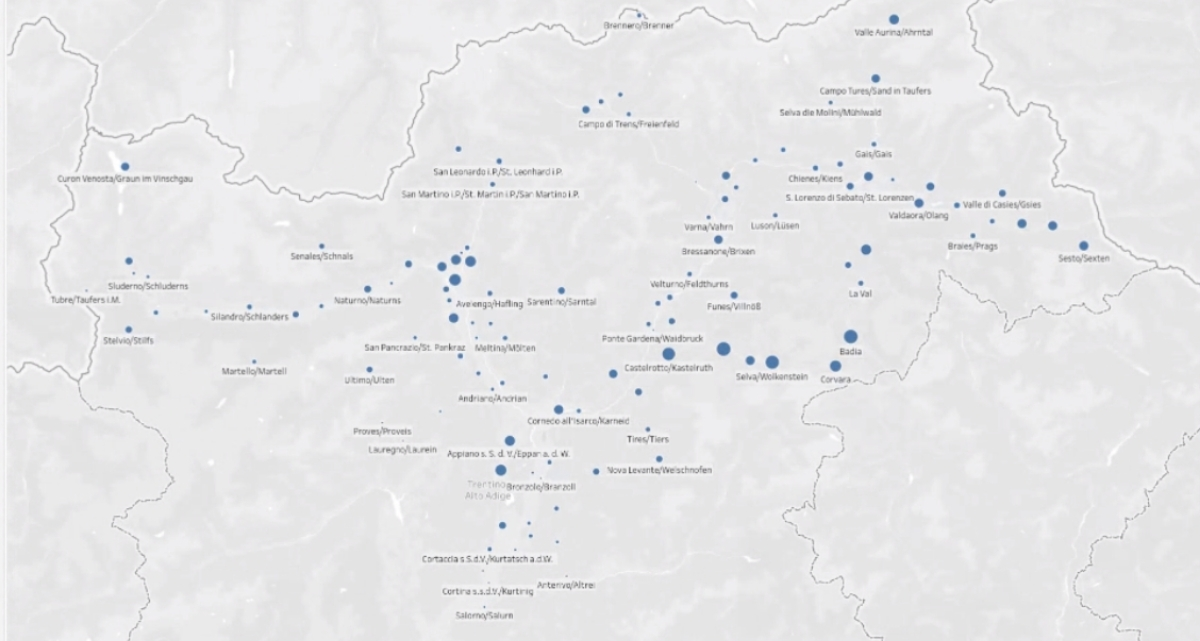
\includegraphics[width = 0.9\linewidth]{MunicipalitiesAltitude.jpg}
    \caption{Distribuzione comuni dell'Alto Adige dove la grandezza è correlata con l'altitudine media}
    \label{fig:MunicipalitiesAltitude}
\end{figure}
\begin{figure}[ht]
    \centering
    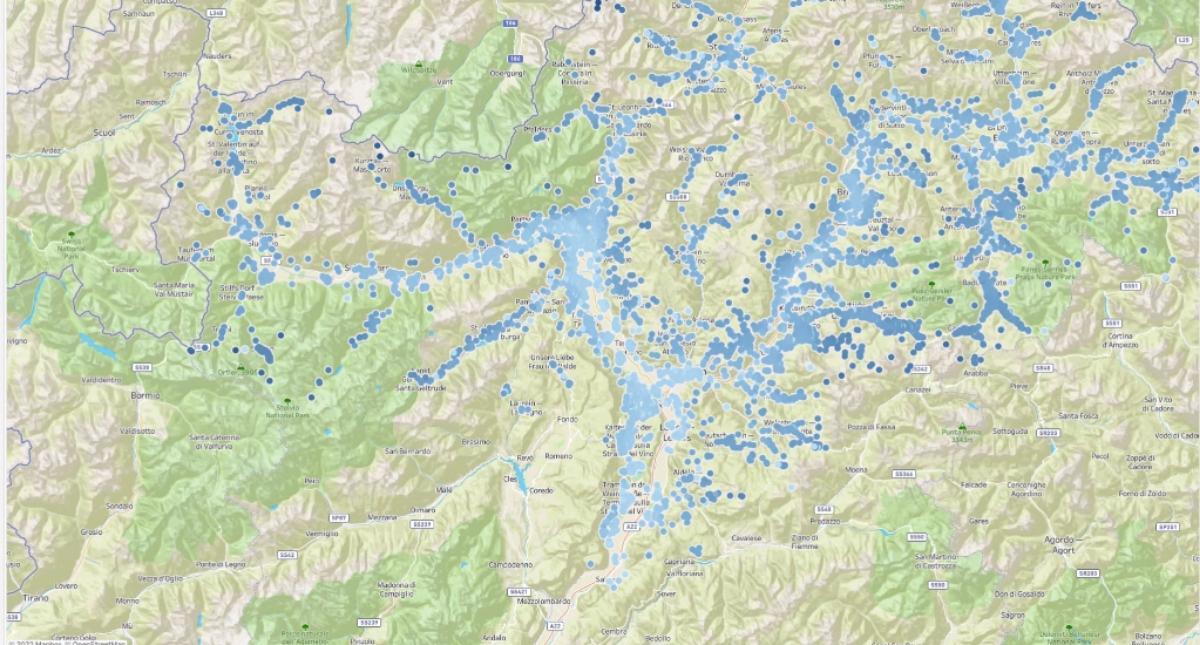
\includegraphics[width = 0.9\linewidth]{HotelsMap.jpg}
    \caption{Distribuzione strutture alberghiere colorate in base alla loro altitudine}
    \label{fig:HotelsMap}
\end{figure}
\begin{figure}[ht]
    \centering
    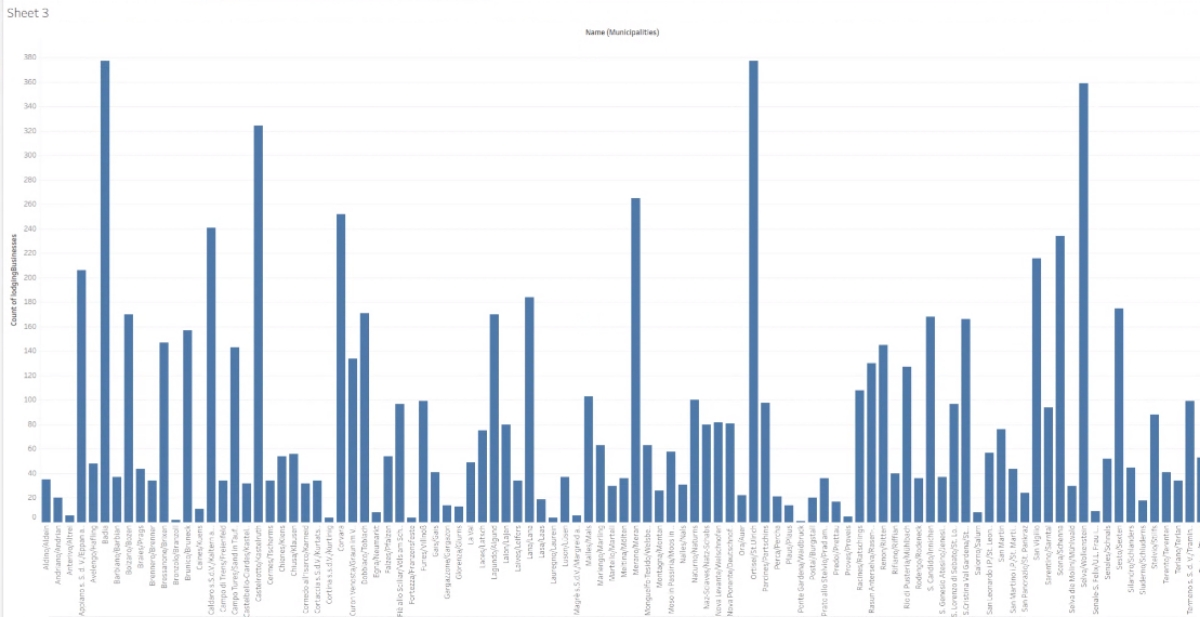
\includegraphics[width = 0.9\linewidth]{HotelsPerMunicipality.jpg}
    \caption{Numero di strutture alberghiere per comune}
    \label{fig:HotelsMunicipality}
\end{figure}